% !TEX root = ../main.tex

\section{Appendix}
\appendix

\section{CryptoKitty} \label{app:cryptokitty}

%Possibly remove this figure due to page limit
\begin{figure}[!htb]
\centering
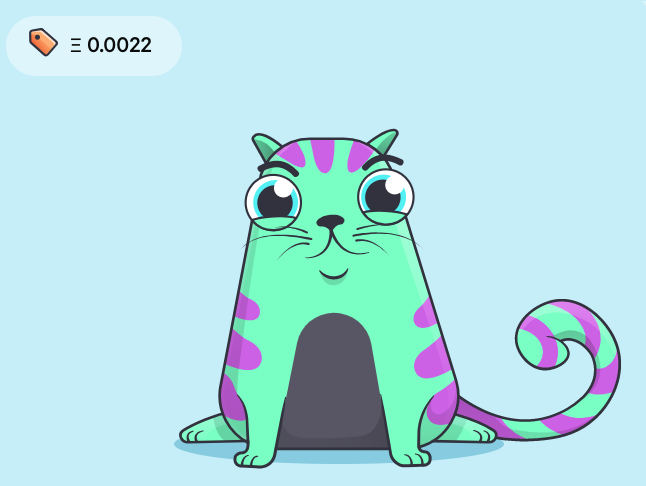
\includegraphics[width=0.3\linewidth]{figures/cryptokittie842912.png}
\caption{ Cryptokitty Number 842912 \label{fig:cryptokittie}}
\end{figure}

Figure~\ref{fig:cryptokittie} shows an example of a Cryptokitty.


\section{LocalEthereum} \label{app:localethereum}

%Possibly remove this code snippet due to page limit . don't forget to remove the refrence to it ^
\begin{lstlisting}[basicstyle=\scriptsize\ttfamily,caption={Code snippet from LocalEthereum smart contract. Values V,R and S are set by LocalEtherem to have a valid signature, also the tradeHash uses buyer and seller addresses, mitigating the possibility of front-running by a third party.},label={code:localethereum}]
    function createEscrow(bytes16 _tradeID, address _seller, address _buyer, uint256 _value, uint16 _fee,
					uint32 _paymentWindowInSeconds, uint32 _expiry, uint8 _v, bytes32 _r, bytes32 _s) 
        payable external {
        bytes32 _tradeHash = keccak256(abi.encodePacked(_tradeID, _seller, _buyer, _value, _fee));
	...
        // A signature (v, r and s) must come from localethereum to open an escrow
        bytes32 _invitationHash = keccak256(abi.encodePacked(
            _tradeHash,
            _paymentWindowInSeconds,
            _expiry
        )); 
\end{lstlisting}

Code~\ref{code:localethereum} shows a mitigation technique employed by LocalEthereum. \\



\section{Traditional Front-running Prevention Methods} \label{app:traditionalprevention}

There are debates in traditional markets regarding the fact that front-running is considered to be a form of insider trading which deemed to be illegal. Traditional methods to prevent front-running mainly involves after the fact investigation and legal action against the front-runners~\cite{LexisNexisLawSuit}. As mentioned in section~\ref{traditionalFrontrunning}, defining front-running and educating the employees were the first step taken to prevent such issues in traditional markets, however, front-running became less likely to happen mainly because of the high fine and lawsuits against firms who behaved in an unethical way. Other methods such as dark pools~\cite{zhu2014dark,buti2011diving} and sealed bids~\cite{radner1989sealed} were discussed and implemented in a variety of regulated trading systems. The traditional methods to prevent front-running does not apply to blockchain applications, as mainly they are based on central enforcement and limitations, also in case of blockchains the actors who are front-running could be anonymous and the fear of lawsuits would not apply. 


\section{Commit-and-Reveal} \label{app:cr}

\begin{figure}[!htb]
\centering
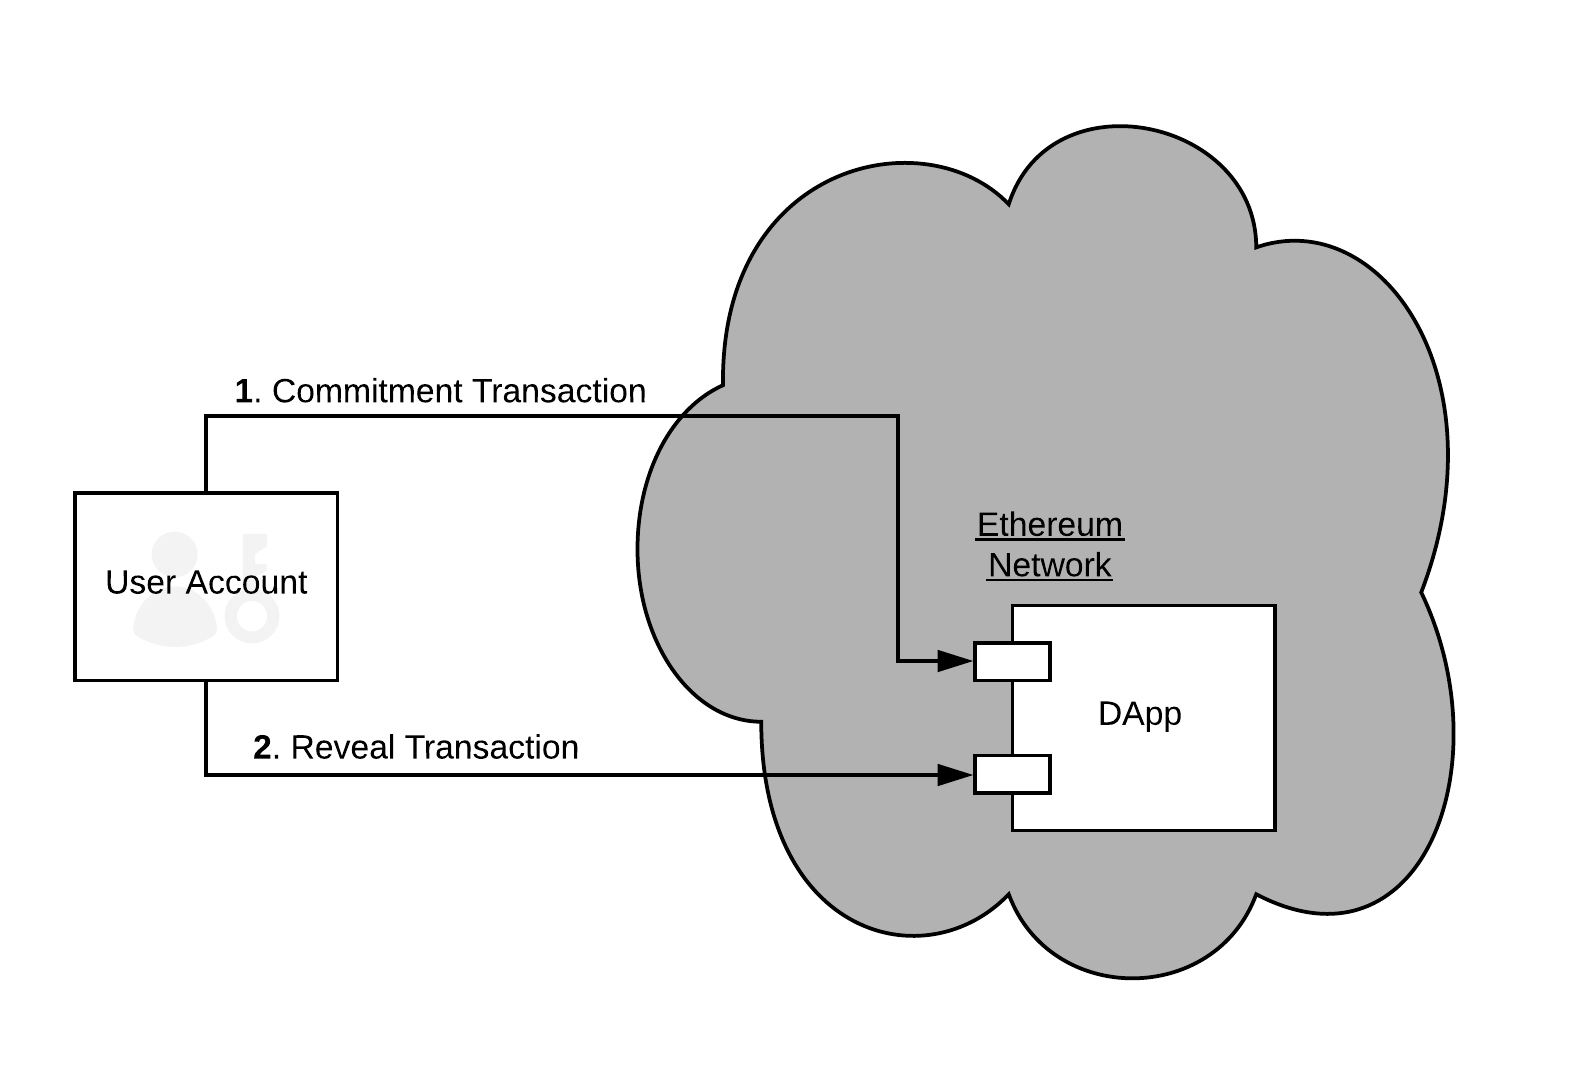
\includegraphics[width=0.5\linewidth]{figures/commit-reveal.png}
\caption{\scriptsize Commit and Reveal. User sends a commitment transaction with the hash of the data, After the commitment period is over, user sends her reveal transaction to the DApp revealing the information that matches the commitment. \label{fig:commitReveal}}
\end{figure}
%https://www.lucidchart.com/invitations/accept/3cd4c865-83d4-4c71-9a4a-f2e870f2db2c

Figure~\ref{fig:commitReveal} illustrates the commit/reveal approach.

